\chapterauthor{Jeferson J. Lima}{Departamento de Informática (DAINF) \\Universidade Tecnológica Federal do Paraná (UTFPR)}
\chapter{Cinemática e Dinâmica de Robôs Móveis com Rodas}


\section{Introdução}\label{intro}

A humanidade é fascinada pelo movimento das rodas a milhares de anos, isso intriga o homem moderno até os dias de hoje. Na matemática, existem áreas específicas para descrever o movimento dos corpos. Um modelo cinemático de um robô com rodas ou pernas, descreve as relações geométricas entre o chassi do robô, seus atuadores e a sua superfície de contato.

Neste capítulo, primeiramente, serão apresentados conceitos sobre a descrição das coordenadas do sistema robótico. 

Na sequência será demonstrada a metodologia para modelagem cinemática dos sistemas, modelos cinemáticos estão relacionadas a como as velocidades dos elementos do robô.

Por fim, será apresentado um exemplo de modelagem cinemática de um robô diferencial.

\section{Rotação, Translação e Transformação Homogênea}\label{rotacao}
 
Para representação de posicionamento e orientação de um sistema de coordenadas faz-se necessário seguir a metodologia do sistema universal de coordenadas.

De acordo com \cite{craig2009introduction} uma vez estabelecido o sistema de coordenada como um vetor de posição $\mathbb{R}^{3 \times 1}$, composto pelas coordenadas $X,Y$ e $Z$, podemos então representar os operadores de rotação, translação e transformação homogênea como operações matriciais. Desta forma, um ponto ${}^A\mathbf{P}$ representa a distância ao longo dos eixos do plano $\{A\}$. Os elementos individuais de ${}^A\mathbf{P}$ podem ser visto pela \eq{eq:cine1}.

\begin{equation}\label{eq:cine1}
    {}^A\mathbf{P} = \begin{bmatrix}
    p_x\\ p_y \\ p_z
    \end{bmatrix}.
\end{equation}

A representação gráfica de ${}^A\mathbf{P}$ pode ser vista na \fig{fig:cine1f}. 

\begin{figure}[!ht]
  \centering
  \begin{tikzpicture}[scale=0.8]
      \node(p0) at (0,0){};
      \draw [->] (p0.center) --++(0,3) node[right] {$ Y_A$};
      \draw [->, rotate =120] (p0.center) --++(0,3) node[below] {$ Z_A$};
      \draw [->, rotate =240] (p0.center) --++(0,3) node[below] {$ X_A$};
      \draw [->, blue] (p0.center) --++(1.5,3.0) node(B)[above,rotate=0] {$\mathbf{P}$};
      \node at (-1.5,2.5) {$\{A\}$};
  \end{tikzpicture}
  \caption{Vetor em relação ao plano $\{A\}$}
  \label{fig:cine1f}
\end{figure}

Além da definição das coordenadas de um vetor, torna-se necessário definir a orientação de um corpo no espaço. O vetor definido por ${}^A\mathbf{P}$ pode ser rotacionado pelo operador de rotação $\mathbf{R}$, demostrado na \eq{eq:cine2}.
 
\begin{equation}\label{eq:cine2}
    {}_A^B
    \mathbf{R} = 
    \begin{bmatrix}
    r_{11} & r_{11} & r_{11}\\
    r_{21} & r_{21} & r_{21}\\
    r_{31} & r_{31} & r_{31}\\
    \end{bmatrix}
\end{equation}

Na \fig{fig:vetor_rot}, a posição de ${}^A\mathbf{P}$ (sistema de referência global) em relação a ${}^B\mathbf{P}$ é encontrado através da multiplicação da matriz de ${}_B^A \mathbf{R}(\theta)$ (lê-se rotação do sistema de referência $B$ em $A$) pela posição de ${}^B\mathbf{P}$.

\begin{figure}[!ht]
    \centering
    \begin{tikzpicture}[scale=0.8]
        \node(p0) at (0,0){};
        \draw [->,] (p0.center) --++(0,3) node[right, yshift=10] {$\hat Y_A$};
        \draw [->, rotate =120] (p0.center) --++(0,3) node[below] {$\hat Z_A$};
        \draw [->, rotate =240] (p0.center) --++(0,3) node[below] {$\hat X_A$};
        \draw [->, rotate =-10, gray] (p0.center) --++(1.5,2) node(A)[above,rotate=0] {${}^A\mathbf{P}$};
        \node(p1) at (6,1){};
        \draw [->, rotate =30, red] (p0.center) --++(0,3) node[right,rotate=30] {$\hat Y_B$};
        \draw [->, rotate =150, red] (p0.center) --++(0,3) node[below,rotate=30] {$\hat Z_B$};
        \draw [->, rotate =270, red] (p0.center) --++(0,3) node[below,rotate=30] {$\hat X_B$};
        \draw [->, rotate =20, red] (p0.center) --++(1.5,2) node(B)[above,rotate=0] {${}^B\mathbf{P}$};
    \end{tikzpicture}
    \caption{Rotação no plano $\{A\}$}
    \label{fig:vetor_rot}
\end{figure}
    
A rotação pode acontecer tanto em $x, y$ ou $z$, conforme é mostrado na \eq{eq:rotxyz}.

\begin{equation}
\begin{split}
    \mathbf{R}_x(\psi) =
    \begin{bmatrix}
        1 & 0            & 0             \\
        0 & \cos(\psi) & -\sin(\psi) \\
        0 & \sin(\psi) & \cos(\psi)  \\
    \end{bmatrix} \text{, eixo $x$ fixo}
    \\    
    \mathbf{R}_y(\phi) =
    \begin{bmatrix}
        \cos(\phi)  & 0 & \sin(\phi) \\
        0             & 1 & 0            \\
        -\sin(\phi) & 0 & \cos(\phi) \\
    \end{bmatrix} \text{, eixo $y$ fixo}
    \\
    \mathbf{R}_z(\theta) =
    \begin{bmatrix}
        \cos(\theta) & -\sin(\theta) & 0 \\
        \sin(\theta) & \cos(\theta) & 0 \\
        0            & 0            & 1 \\
    \end{bmatrix} \text{, eixo $z$ fixo}
\end{split}
\label{eq:rotxyz}
\end{equation}

Além do operador de rotação ($\mathbf{R}$), pode-se aplicar um deslocamento entre os planos, deslocamento aqui demostrado por $\mathbf{Q}$. A este deslocamento dá se o nome de translação, onde a translação é executada pelo operador translacional $\mathbf{D}_A(q)$. Utilizará-se da notação ${}^A\mathbf{Q}$ para representa uma translação entre os planos $\{A\}$ e $\{B\}$, conforme \eq{eq:cine4}.

\begin{equation}\label{eq:cine4}
    {}^A\mathbf{Q} =
    \begin{bmatrix}
    q_x\\ q_y \\ q_z
    \end{bmatrix}, \qquad
    \mathbf{D}_A = 
    \begin{bmatrix}
    \mathbf{I} & \mathbf{Q}\\
    0 & 1\\
    \end{bmatrix}, \mathrm{ou} \qquad
    \mathbf{D}_A = 
    \begin{bmatrix}
    1 & 0 & 0 & q_x\\
    0 & 1 & 0 & q_y\\
    0 & 0 & 1 & q_z\\
    0 & 0 & 0 & 1
    \end{bmatrix}.
\end{equation}
    
Adota-se agora a notação para translação e rotação de um vetor, conforme a \eq{eq:cine5}. Pode-se concluir pela \eq{eq:cine5}, que $\mathbf{D}_A$, descrito na \eq{eq:cine4}, representa a operação da \eq{eq:cine5} com ângulo de rotação zero.
    
\begin{equation}\label{eq:cine5}
    \begin{bmatrix}
        {}^B_A\mathbf{P}\\ 1
    \end{bmatrix}
    =
    \underbrace {
    \left[
    \begin{matrix}
        & {}_B^A\mathbf{R}& \\ \hline
        0 & 0 & 0\\
    \end{matrix} \right.
    \left.
    \vline
    \begin{matrix}
        {}^A\mathbf{Q}\\ \hline
        1
    \end{matrix} \right]
    }_{{}^A_B\mathcal{A}}
    \begin{bmatrix}
        {}^B\mathbf{P}\\
        1
    \end{bmatrix}
\end{equation}
    
Na \eq{eq:cine5} a matriz ${}^A_B\mathcal{A}$ representa a matriz de transformação homogênea, neste caso, composta pela matriz de rotação ${}^A_B \mathbf{R}$ e de translação ${}^A\mathbf{Q}$. Pode-se ver graficamente o resultado da operação da \eq{eq:cine5} pela \fig{fig:cine2}.
    
\begin{figure}[!ht]
    \centering
    \begin{tikzpicture}
        \node(p0) at (0,0){};
        \draw [->] (p0.center) --++(0,3) node[right] {$\hat Y_A$};
        \draw [->, rotate =120] (p0.center) --++(0,3) node[below] {$\hat Z_A$};
        \draw [->, rotate =240] (p0.center) --++(0,3) node[below] {$\hat X_A$};
        \draw [->, blue] (p0.center) --++(1.5,4) node(B)[above,rotate=30] {$\mathbf{P}$};
        \node(p1) at (6,1){};
        \draw [->, rotate =30] (p1.center) --++(0,3) node[right,rotate=30] {$\hat Y_B$};
        \draw [->, rotate =150] (p1.center) --++(0,3) node[below,rotate=30] {$\hat Z_B$};
        \draw [->, rotate =270] (p1.center) --++(0,3) node[below,rotate=30] {$\hat X_B$};
        \draw [->, blue] (p1.center) --++(-0.5,4.5) node(B)[above,rotate=30] {$\mathbf{P}$};
        \draw [dotted,-latex] (p0)  -- (p1) node[midway, fill=white]{${}^A\mathbf{Q}$};
        \draw [dotted] (p0)  -- (B);
        \node at (-1.5,2.5) {$\{A\}$};
        \node at (4,2.5)  [rotate=30]   {$\{B\}$};
    \end{tikzpicture}
    \caption{Transformação homogênea do ponto ${}^A\mathbf{P}$ pelos operadores de rotação e translação.}
    \label{fig:cine2}
\end{figure}

Na forma generalizada, a transformação homogênea ${}^{i}_0\mathbf{T}$ pode ser expressa por produto das sucessivas transformações de ${}^{i-1}_0\mathcal{A}_i$. Conforme é mostrado na \eq{fig:cine3}.

\begin{equation}\label{fig:cine3}
    \begin{array}{lcl}
        {}^i_0\mathbf{T} &= & {}^0_1\mathcal{A}{}^1_2\mathcal{A} \cdots {}^{i-1}_i\mathcal{A} = \prod \limits^i_{j=1}{}^{j-1}_i\mathcal{A}, \quad \mathrm{para\;}i=1,2,\cdots,n\\[.2cm]
        & = &
    \begin{bmatrix}
        x_i & y_i & z_i & p_i\\
        0 & 0 & 0 & 1
    \end{bmatrix} = 
    \begin{bmatrix}
        {}^i_0\mathbf{R} & {}^i_0\mathcal{P}\\
        \mathbf{0} & 1
    \end{bmatrix}
    \end{array}
\end{equation}
    
\noindent onde, ${}^i_0\mathcal{P}$ é o vetor de orientação do referencial $i$ em relação à base em  $0$.


\section{Conceitos de Cinemática}\label{intro-ch1}

Como exposto anteriormente, a cinemática é a ciência que trata do movimento e forças que o causam, \cite{craig2009introduction, klancar2017wheeled}. Desta forma, podemos definir o sistema de referências do robô pela cinemática externa ou interna. 

A cinemática externa referência as velocidades do sistema em relação a coordenadas externas ao robô, a \fig{fig:cardes}, onde o robô em $\{B\}$ tem seu sistema de referência fixado em $\{A\}$. Este sistema de referência  pode ser compreendida como a relação entre o robô e as coordenadas de um mapa global, por exemplo.

\begin{figure}[!ht]
    \centering
    \input{chapters/chapter1/figures/car_1_image.tex}
    \caption{Robô Diferencial em $\{B\}$, reapresentação do Mapa em $\{A\}$.}
    \label{fig:cardes}
\end{figure}

Quando o próprio robô é o sistema de referência, da-se o nome de cinemática interna. 
Podemos ainda nos aprofundar mais sobre a cinemática Interna do robô, será utilizado modelo braço robótico demonstrado na \fig{fig:2dof-robot}.

\begin{figure}[!ht]


\begin{tikzpicture}
    \newcommand{\nvar}[2]{%
    \newlength{#1}
    \setlength{#1}{#2}
    }

    % Define a few constants for drawing
    \nvar{\dg}{0.3cm}
    \def\dw{0.25}\def\dh{0.5}
    % Define commands for links, joints and such
    \def\link{\draw [double distance=1.5mm, very thick] (0,0)--}
    \def\joint{%
    \filldraw [fill=white] (0,0) circle (5pt);
    \fill[black] circle (2pt);
    }
    \def\grip{%
    \draw[ultra thick, blue](0cm,\dg)--(0cm,-\dg);
    \fill[blue] (0cm, 0.5\dg)+(0cm,1.5pt) -- +(0.6\dg,0cm) -- +(0pt,-1.5pt);
    \fill[blue] (0cm, -0.5\dg)+(0cm,1.5pt) -- +(0.6\dg,0cm) -- +(0pt,-1.5pt);
    }

    \def\robotbase{%
    \draw[rounded corners=8pt] (-\dw,-\dh)-- (-\dw, 0) --
        (0,\dh)--(\dw,0)--(\dw,-\dh);
    \draw (-0.5,-\dh)-- (0.5,-\dh);
    \fill[pattern=north east lines] (-0.5,-1) rectangle (0.5,-\dh);
    }
    \newcommand{\doublelink}[6]{%
    \robotbase
    \link(#1:#2);
    \joint
    \node[left]{$\color{black}{\theta_1}$};
    \begin{scope}[shift=(#1:#2), rotate=#1]
        \link(#3:#4);
        \joint
        \node[above]{$\color{black}{\theta_2}$};
        \begin{scope}[shift=(#3:#4), rotate=#5]
            \grip
            \node[right]{$\color{blue}{\mathbf{x}_{tool}}$};
        \end{scope}
    \end{scope}
    }

    \doublelink{60}{2}{-90}{2}{-60}{1}
\end{tikzpicture}
    
\caption{Robô - Dois Graus de Liberdade}
\label{fig:2dof-robot}
\end{figure}

Para o robô fixo da \fig{fig:2dof-robot}, as coordenadas generalizadas $\theta_1, \theta_2,..., \theta_n$ descrevem o chamado espaço das \textcolor{red}{juntas ou atuadores (\textit{joint space}) $\mathbf{q}$}. Bem como $x_1, x_2,..., x_n$, o \textcolor{blue}{espaço das tarefas (\textit{task space}) $\mathbf{x}$}.

Outro termo a ser apresentado é o de cinemática direta e cinemática inversa. Da-se o nome de a \textcolor{red}{cinemática direta} quando o robô é descrito em função de entradas, como a velocidade das rodas, movimento das juntas, direção das rodas, etc. Já a \textcolor{blue}{cinemática inversa} nos possibilita projetar um planejamento de movimento do elemento final do manipulador $\textcolor{blue}{\mathbf{x}_f}$, como no exemplo da \fig{fig:2dof-robot}.

A relação entre as cinemáticas direta e cinemática inversa é obtida através da Matriz Jacobiana, conforme demonstrado na \eq{eq:jac01}, \eq{eq:jac02} e \eq{eq:jac03}.

\begin{equation}
    \mathbf{\dot{x}} = \mathbb{J}{\mathbf{\dot{q}}}
    \text{ e, }
    \mathbf{\dot{q}} = \mathbb{J}^{-1}{\mathbf{\dot{x}}}
    \label{eq:jac01}
\end{equation}

\noindent bem como:

\begin{equation}
    \frac{\text{d}\mathbf{x}}{\text{d}t} = \mathbb{J}\frac{\text{d}\mathbf{q}}{\text{d}t}
    \text{ e, }
    \frac{\text{d}\mathbf{q}}{\text{d}t} = \mathbb{J}^{-1}\frac{\text{d}\mathbf{x}}{\text{d}t}
    \label{eq:jac02}
\end{equation}

\noindent onde $\mathbb{J}$ é dado por:

\begin{equation}
    \mathbb{J}
    =
    \frac{d \mathbf{f}}{d \mathbf{q}}
    =
    \left[ \frac{\partial \mathbf{f}}{\partial q_1}
        \cdots \frac{\partial \mathbf{f}}{\partial q_n} \right]
    =
    \begin{bmatrix}
        \frac{\partial f_1}{\partial q_1} & \cdots &
        \frac{\partial f_1}{\partial q_n}                   \\
        \vdots                            & \ddots & \vdots \\
        \frac{\partial f_m}{\partial q_1} & \cdots &
        \frac{\partial f_m}{\partial q_n}
    \end{bmatrix}
    \label{eq:jac03}
\end{equation}

A matriz jacobiana viabiliza o processo de controle de um robô utilizando-se, por exemplo, das referências de uma ferramenta acoplada a
extremidade do braço robótico.

\subsection{Cinemática de Robôs Móveis com Rodas}

A Cinemática para Robô com Rodas será apresentada a seguir, no entanto, será necessário adicionar algumas restrições impostas pelo modelo de utilização de determinadas rodas.

Desta forma, a discussão a seguir segue conforme o arranjo de rodas de determinados robôs, sejam estas rodas convencionais, fixas ou castor. A descrição do modelo de roda a será apresentado na sequência.

\subsection{Cinemática Robô Diferencial}

O objeto de estudo nesta sessão será o modelo de Robô Diferencial. Embora o modelo possa ser considerado simples, diante da enorme gama de aplicações, os fundamentos aqui apresentados serão de fácil aplicação as diversas outras propostas de robôs.

Um robô diferencial apresenta uma construção padrão, composta por duas rodas fixas instaladas nas laterais direita e esquerda do chassi do robô. Tipicamente uma roda no formato castor é adicionada ao chassi para dar sustentação ao chassi, no entanto, não apresenta uma restrição considerável ao sistema, desta forma não será inclusa no modelo de restrições do robô diferencial.

A \fig{fig:car01} mostra o robô diferencial descrito pelo sistema de referências $\{R\}$ e $\{M\}$ representa o sistema de referência global, podemos assumir aqui que $\{M\}$ é o mapa onde o robô $\{R\}$ se deslocará.

As variáveis $v_{E}$ e $v_{D}$ representam respectivamente as velocidades da roda esquerda e roda da direita do chassi. A velocidade resultante do robô é expressa por $v_{R}$.
A sigla $\text{CIR}$ representa o ponto do Centro de instantâneo de Rotação. Quanto maior for o ângulo de uma curva, mais próximo teremos o $\text{CIR}$ do centro de massa do robô.

\begin{figure}[!ht]
    \centering
    \def\iangle{35} % Angle of the inclined plane
\def\down{0}
\def\arcr{0.7cm} % Radius of the arc used to indicate angles
\newcommand\centerofmass{%
    \tikz[radius=0.2em] {%
        \fill (0,0) -- ++(0.2em,0) arc [start angle=0,end angle=90] -- ++(0,-0.4em) arc [start angle=270, end angle=180];%
        \draw (0,0) circle;%
    }%
}

\begin{tikzpicture}[
    force/.style={>=latex,draw=blue,fill=blue},
    axis/.style={densely dashed,gray,font=\small},
    M/.style={rectangle,draw,fill=lightgray,minimum size=0.7cm,thin},
    m/.style={rectangle,draw=black,fill=lightgray,minimum size=0.3cm,thin},
    plane/.style={draw=black,fill=blue!10},
    string/.style={draw=red, thick},
    pulley/.style={thick},
    wheel/.style={fill=black, rounded corners=1.5pt},
]
    %% Free body diagram of M
    \begin{scope}[rotate=\iangle]
        \node[M,transform shape] (M) {\centerofmass};
        % Draw axes and help lines
        {[axis,->]
            \draw (M) -- ++(0,1.3) node(y1_axis)[right] {$y$};
            \draw (M) -- ++(2,0) node[right] {$x$};
            % Indicate angle. The code is a bit awkward.
            \draw[solid,shorten >=0.5pt] (\down-\iangle:\arcr)
                arc(\down-\iangle:\down:\arcr);
            \node at (\down-0.5*\iangle:1.3*\arcr) {$\phi$};
        }
        % Forces
        {[force,->]
            % Assuming that Mg = 1. The normal force will therefore be cos(alpha)
            \draw (M.east) -- ++(1,0) node[above, blue] {$v_M$};
        }
        \draw[wheel] (M.south west) rectangle ++(.4,-.1) node[below]{$v_{M_R}$};
        \draw[wheel] (M.north west) rectangle ++(.4,.1)  node[left]{$v_{M_L}$};
        \draw [-](M) -- ++(0,2) node(CIR)[above] {CIR};
    \end{scope}
    % Draw gravity force. The code is put outside the rotated
    % scope for simplicity. No need to do any angle calculations. 
    \draw[axis,] (M.center) -- ++(1,0) node[below] {};
    %%
    \node[right, gray,font=\small, xshift=8] at (y1_axis) {$\{M\}$};
    %%
    \draw[, ->] (-2,-1) -- ++(4,0) node[below] {$X$};
    \draw[, ->] (-2,-1) -- ++(0,3) node(y_axis)[right] {$Y$};
    \draw[gray, ->] (-2,-1) -- ++(-.5,-.5) node[left] {$Z$};
    \node[left, gray,font=\small, xshift=-10] at (y_axis) {$\{I\}$};
\end{tikzpicture}

    \caption{Robô Diferencial.}
    \label{fig:car01}
\end{figure}

Apresentadas as variáveis do sistema é possível agora, deduzir as equações da cinemática do robô diferencial. A variável $\omega$ representará a velocidade de rotação em relação ao $\text{CIR}$, variável $r(t)$ é o raio em relação a cada centro de massa do chassi e $L$ a distância entre as rodas. Podemos então, deduzir a equação da cinemática pela \eq{eq:cinerd1}, \eq{eq:cinerd2}, \eq{eq:cinerd3} e \eq{eq:cinerd4}.

\begin{equation}
    \omega(t) = \frac{v_{E}(t)}{r(t) - \displaystyle\frac{L}{2}}
    \label{eq:cinerd1}
\end{equation}

\noindent bem, como para roda direita:

\begin{equation}
    \omega(t) = \frac{v_{D}(t)}{r(t) + \frac{L}{2}}
    \label{eq:cinerd2}
\end{equation}

Sendo assim, temos as seguintes expressões:

\begin{equation}
    \omega(t) = \frac{v_{D}(t) - v_{E}(t)}{L}, \quad\quad r(t) = \frac{Lv_{D}(t) + v_{E}(t)}{2v_{D}(t) - v_{E}(t)}
    \label{eq:cinerd3}
\end{equation}

Podemos agora definir a velocidade resultante de $v_M$ pela equação

\begin{equation}
    v_R (t) = \omega(t) r(t) = \frac{v_{D}(t) + v_{E}(t)}{2}
    \label{eq:cinerd4}
\end{equation}

Diante das equações listadas acima, pode-se apresentar então o modelo cinemático do robô diferencial $\{R\}$ em relação ao sistema de referências global $\{M\}$, conforme a \eq{eq:cinerd5}.

\begin{equation}
    \begin{bmatrix}
        \dot{X}(t) \\ \dot{Y}(t) \\ \dot{\phi}(t)
    \end{bmatrix}
    =
    \begin{bmatrix}
        \cos(\phi(t)) & 0 \\
        \sin(\phi(t)) & 0 \\
        0             & 1
    \end{bmatrix}
    \begin{bmatrix}
        v_R(t) \\ \omega(t)
    \end{bmatrix}
    \label{eq:cinerd5}
\end{equation}

Bem como, podemos definir as equações da cinemática interna do robô diferencial, expressas pelo sistema referência $\{R\}$. O termo $r_r$ na \eq{eq:cinerd6} diz respeito ao raio das rodas. 

\begin{equation}
    \begin{bmatrix}
        \dot{x}_R(t) \\ \dot{y}_R(t) \\ \dot{\phi}(t)
    \end{bmatrix}
    =
    \begin{bmatrix}
        \frac{r_r}{2} & \frac{r_r}{2} \\
        o & 0 \\
        -\frac{r_r}{L} & \frac{r_r}{L}
    \end{bmatrix}
    \begin{bmatrix}
        \omega_E(t) \\ \omega_D(t)
    \end{bmatrix}
        \label{eq:cinerd6}
\end{equation}

Conforme mostrado na \fig{fig:car01}, algumas restrições de movimento definem a cinemática e dinâmica do robô. No caso da \fig{fig:car01} esta restrição atua em $\dot{y}_R$ onde este sempre, em condições normais, apresentará velocidade igual a zero, conforme a \eq{eq:cinerd6}.

\section{Dinâmica com Restrições de Movimento}

Tipicamente, um robô com rodas apresenta uma série de restrições relacionadas ao seu modelo de construção, como exemplo, fatores relacionados a inércia ou mesmo as características dos atuadores \cite{klancar2017wheeled}.

As restrições da cinemática podem ser classificadas como holonômicas ou não holonômicas. Restrições holonômicas estão relacionadas a dimensionalidade da descrição do estado de um sistema, sendo ele, expresso em coordenadas generalizadas, conforme demonstrado na \fig{fig:2dof-robot}.

Um sistema é considerado holonômico quando não apresenta limitação de velocidades em seus estados. Neste aspecto, podemos considerar o Robô de dois graus de liberdade, apresentado na \fig{fig:2dof-robot}, um sistema holonômico, quando não há restrição de velocidade no robô, ou mesmo de contato.

Já em um sistema não holonômico, tais restrições impedem que o robô, mova em direções arbitrárias. Um exemplo clássico é apresentado na  \fig{fig:car01}, onde o robô diferencial possui restrições ao movimento em $y$.

\subsection{Restrições Holonômicos}

Um sistema holonômico possui restrições dependentes das coordenadas generalizadas, sendo, $n$ coordenadas generalizadas $\mathbf{q} = [q_1, \cdots, q_n]$, conforme a \eq{eq:homo} de restrições de vínculos.

\begin{equation}
    f(\mathbf{q}) = f(q_1, \cdots, q_n) = 0
    \label{eq:homo}
\end{equation}

\noindent a função $f(\mathbf{q})$ e sua derivada são funções contínuas.

Observa-se também que a função da \eq{eq:homo} não depende das velocidades ou de qualquer derivada de ordem superior com relação a $t$. Em geral, podemos ter $m$ restrições holonômicas, ou seja $(m<n)$. 

Assim, como exposto, pode-se agora definir es equações de energia que regem o sistema de um robô. A formulação de Lagrange, apresentada na \eq{eq:lag1} introduz o funcional relacionado as energias conservativas do sistema. Em $\mathcal{T}$ temos a composição de energias cinéticas e em $\mathcal{V}$ as energias potenciais.

\begin{equation}
    \mathcal{L}= \mathcal{T} - \mathcal{V}
    \label{eq:lag1}
\end{equation}

A equação de energia cinética ($\mathcal{T}$) é dada pela \eq{eq:lag2}, onde os termos $\mathbf{M}_k$ representa as massas associadas aos $k$ elementos do sistema de equação de movimento. Já $\mathbf{J}_k $ inclui as forças e inércia relacionadas aos sistemas rotativos.

\begin{equation}
  \mathcal{T} = \frac{1}{2} \sum\limits_{k=1}^{N}{\mathbf{\dot{q}}_k}^T  \mathbf{M}_k {\mathbf{\dot{q}}_k}+ \frac{1}{2} \sum\limits_{k=1}^{N}\mathbf{\omega}_k^T \mathbf{J}_k \mathbf{\omega}_k
  \label{eq:lag2}
\end{equation}

A equação de Energia Potencial ($\mathcal{V}$) pode assumir várias formas, dependendo do tipo de energia potência ao qual o sistema robótico está incluso. Apresenta-se aqui o caso da energia Potencial Gravitacional, aplicável na \fig{fig:2dof-robot}, definida por $\mathcal{V}_g$, conforme eq{eq:lag3}.

\begin{equation}
  \mathcal{V}_g = \sum\limits_{k=1}^{N}\mathbf{M}g \underbrace{\Delta y_k}_{\text{altura}}
  \label{eq:lag3}
\end{equation}  

\noindent onde

\begin{center}
   \begin{tabular}{l|l}
       $\mathbf{M}$               & Massa     \\
       $\mathbf{\omega}$ & Velocidade Angular \\
       $\mathbf{J}$               & Inércia   \\
   \end{tabular}
\end{center}

Desta forma, pode-se propor a Formulação do Lagrange, conforme \eq{eq:lag4}.
\begin{equation}
   \frac{d}{\df{t}}\left( \parcial{}{\mathcal{L}}{\dot{q}_k}\right)
   -\parcial{}{\mathcal{L}}{q_k}
   = f_k, \quad k = 1,2,...,n
   \label{eq:lag4}
\end{equation}

\noindent onde $k$ é o índice das coordenadas generalizadas de $g_k$, $f_k$ são as forças externas que agem no sistema.

O modelo dinâmico de um robô móvel sem restrições de movimento pode ser expresso pelo \eq{eq:lag5}.

\begin{equation}
   \mathbf{M(q)\ddot{q}+ C(q, \dot{q})+ \textcolor{red}{F(\dot{q})}+G(q) = E(q)u}
   \label{eq:lag5}
\end{equation}

\noindent onde, 

\begin{center}
   \begin{tabular}{ r | l }
     $\mathbf{q}$               & Vetor das coordenadas generalizadas    \\
     $\mathbf{M(q)}$            & Matriz de massa e inércia              \\
     $\mathbf{C(q, \dot{q})}$   & Vetor de força Coriolis e centrifuga   \\
     $\color{red}{\mathbf{F(\dot{q})}}$      & Vetor de atrito, força não conservativa\\
     $\mathbf{G(q)}$            & Vector da força gravitacional          \\
     $\mathbf{E(q)}$            & Matriz de transformação dos atuadores \\
     $\mathbf{u}$               & Vetor de entrada do sistema            \\
   \end{tabular}
\end{center}

A solução numérica pode ser encontrada através da integração da aceleração ($\mathbf{\ddot{q}}$), conforme \eq{eq:accel}.

\begin{equation}
   \mathbf{\ddot{q}}=\mathbf{M(q)}^{-1}\left\{\mathbf{-C(q, \dot{q})-F(\dot{q})-G(q) + E(q)u}\right\}
   \label{eq:accel}
\end{equation}

Porém, aplicações de robótica móvel, como o exemplo do robô diferencial, possuem algumas restrições ao movimento. Tais restrições, onde o número de restrições é superior ao grau de liberdade do sistema $(m>n)$, classificam o sistema com Não-Holonômicos. Assim, faz se necessário incluir estas restrições no modelo, conforme será visto na próxima sessão.

\subsection{Sistemas Não-Holonômicos}

Analogicamente ao Sistema Holonômicos, apresentados na anteriormente, Sistemas Não-Holonômicos possuem restrições de vínculo, bem como, restrições de velocidade do sistema. Podemos reformular equação de restrições conforme mostrado pela \eq{eq:nonhomo}.

\begin{equation}
    f(\mathbf{q}, \dot{\mathbf{q}}) = f(q_1, \cdots, q_n, \dot{q}_1, \cdots, \dot{q}_n) = 0
    \label{eq:nonhomo}
\end{equation}

As restrições cinemáticas apresentadas pela \eq{eq:nonhomo}, representam um sistema holonômico, conforme \cite{klancar2017wheeled}, se $f(\mathbf{q}, \dot{\mathbf{q}})$ for integrável, ou seja, possibilitando com que as velocidades $\dot{q}_k$ sejam eliminadas da equação, podendo assim, a \eq{eq:nonhomo} ser expressa na forma de \eq{eq:homo}.

Tais restrições, com já comentado, estão diretamente associadas as modelos de rodas utilizas no projeto de robô móvel. A \fig{fig:rodas} demonstra a variedade de opções. Cada modelo, impõe uma restrição que poderá ser descrita geometricamente.

\begin{figure}[!ht]
    \centering
    \includegraphics[width=0.5\textwidth]{chapters/chapter1/figures/tipo_de_rodas.png}
    \caption{Rodas (a) Convencionais (b) Castor (c) Sueca (d) Esférica. \\
    Fonte: Adaptado de \cite{klancar2017wheeled}.}
    \label{fig:rodas}
\end{figure}

 Definidas os tipos de rodas e restrições ao sistema, podemos então propor o modelo dinâmico do robô diferencial, mostrado na \fig{fig:car01}.

\subsection{Dinâmica do Robô Diferencial}

Como já discutido, as restrições impostas pelas rodas convencionais, fixadas nas laterais do chassi possibilitam a locomoção apenas no eixo $x$, conforme demonstrado na \fig{fig:car01}. Diante disto, tem-se o modelo cinemático do robô diferencial na \eq{eq:modcinematico}.

\begin{equation}
    \begin{bmatrix}
        \dot{X}(t) \\ \dot{Y}(t) \\ \dot{\phi}(t)
    \end{bmatrix}
    =
    \begin{bmatrix}
        \cos(\phi(t)) & 0 \\
        \sin(\phi(t)) & 0 \\
        0             & 1
    \end{bmatrix}
    \begin{bmatrix}
        v_R(t) \\ \omega(t)
    \end{bmatrix}
    \label{eq:modcinematico}
\end{equation}

Sujeito as restrições de movimento impostas pelo modelo de roda fixa, conforme \fig{fig:rodas}, restrições descritas pela \eq{eq:rstricoes}.

\begin{equation}
    -\dot{x}\sin(\phi) + \dot{y}\cos(\phi) = 0
    \label{eq:rstricoes}
\end{equation}

\noindent ou na forma matricial, as restrições são expressas por $\textbf{A}$, conforme:

\begin{equation}
    \mathbf{A} = 
    \begin{bmatrix}
        - \sin(\phi) & \cos(\phi) & 0
    \end{bmatrix}
    \label{eq:rstricoesmat}
\end{equation}

De forma análoga, a \fig{fig:gocar} nos mostra as possibilidades deslocamento do Robô diferencial, bem como, percebe-se que o vetor de movimento $v'$ não é uma opção valida, diante das restrições das rodas.

\begin{figure}[!ht]
    \centering
    \def\iangle{35} % Angle of the inclined plane
\def\down{0}
\def\arcr{0.7cm} % Radius of the arc used to indicate angles
\newcommand\centerofmass{%
    \tikz[radius=0.2em] {%
        \fill (0,0) -- ++(0.2em,0) arc [start angle=0,end angle=90] -- ++(0,-0.4em) arc [start angle=270, end angle=180];%
        \draw (0,0) circle;%
    }%
}

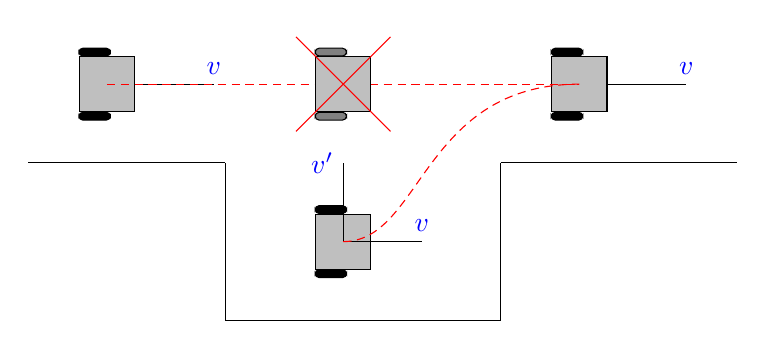
\begin{tikzpicture}[
    force/.style={>=latex,draw=blue,fill=blue},
    axis/.style={densely dashed,gray,font=\small},
    M/.style={rectangle,draw,fill=lightgray,minimum size=0.7cm,thin},
    m/.style={rectangle,draw=black,fill=lightgray,minimum size=0.3cm,thin},
    plane/.style={draw=black,fill=blue!10},
    string/.style={draw=red, thick},
    pulley/.style={thick},
    wheel/.style={fill=black, rounded corners=1.5pt},
]
     \begin{scope}[rotate=0]
        \node[M,transform shape] (M1) at (0,0) {\centerofmass};
        % Draw axes and help lines
        % Forces
        {[force,->]
            % Assuming that Mg = 1. The normal force will therefore be cos(alpha)
            \draw (M1.east) -- ++(1,0) node[above, blue] {$v$};
        }

        \draw[wheel,] (M1.south west) rectangle ++(.4,-.1) node[]{};
        \draw[wheel,] (M1.north west) rectangle ++(.4,.1)  node[]{};
    \end{scope}


    \begin{scope}[rotate=0]
        \node[M,transform shape] (M2) at (6,0) {\centerofmass};
        % Draw axes and help lines
        % Forces
        {[force,->]
            % Assuming that Mg = 1. The normal force will therefore be cos(alpha)
            \draw (M2.east) -- ++(1,0) node[above, blue] {$v$};
        }

        \draw[wheel,] (M2.south west) rectangle ++(.4,-.1) node[]{};
        \draw[wheel,] (M2.north west) rectangle ++(.4,.1)  node[]{};
    \end{scope}
    \begin{scope}[rotate=0]
        \node[M,transform shape] (M3) at (3,-2) {\centerofmass};
        % Draw axes and help lines
        % Forces
        {[force,->]
            % Assuming that Mg = 1. The normal force will therefore be cos(alpha)
            \draw (M3.center) -- ++(1,0) node[above, blue] {$v$};
            \draw (M3.center) -- ++(0,1) node[left, blue] {$v'$};
        }

        \draw[wheel,] (M3.south west) rectangle ++(.4,-.1) node[]{};
        \draw[wheel,] (M3.north west) rectangle ++(.4,.1)  node[]{};
    \end{scope}

%%
    \draw (-1,-1)           -- ++(2.5,0) node[](wall_1){};
    \draw (wall_1.center)   -- ++(0,-2) node[](wall_2){};
    \draw (wall_2.center)   -- ++(3.5,0) node[](wall_3){};
    \draw (wall_3.center)   -- ++(0,2) node[](wall_4){};
    \draw (wall_4.center)   -- ++(3,0) node[](wall_4){};    

    \draw[densely dashed, red] (M1.center) -- (M2.center);

    \begin{scope}[rotate=0]
        \node[M,transform shape] (M4) at (3,0) {\centerofmass};
        % Draw axes and help lines
        % Forces

        \draw[wheel,fill=gray] (M4.south west) rectangle ++(.4,-.1) node[]{};
        \draw[wheel,fill=gray] (M4.north west) rectangle ++(.4,.1)  node[]{};

        \draw[red] (3,0) -- ++(-0.6,-0.6) node[]{};
        \draw[red] (3,0) -- ++(0.6,-0.6) node[]{};
        \draw[red] (3,0) -- ++(-0.6,0.6) node[]{};
        \draw[red] (3,0) -- ++(0.6,0.6) node[]{};
    \end{scope}

    \draw[densely dashed, red] (M3.center) .. controls ++(1,0) and ++(-2,0) .. (M2.center);

    % Draw gravity force. The code is put outside the rotated
    % scope for simplicity. No need to do any angle calculations. 
\end{tikzpicture}

    \caption{Restrições de Movimento das Rodas do Robô Diferencial}
    \label{fig:gocar}
\end{figure}

Apresentadas as restrições, pode-se então, propor o sistema dinâmico do robô diferencial inciando pela Formulação de Lagrange.

\begin{equation*}
    \mathcal{L}= \mathcal{T} - \mathcal{V}
\end{equation*}

A equação de energia cinética ($\mathcal{T}$) é dada por:

\begin{equation}
    \mathcal{T} = \sum\limits_{i=0}^{N-1} \frac{1}{2} {}_{i}^{i+1}\dot{\mathbf{P}}^T\cdot m_{i}\cdot {}_{i}^{i+1}\dot{\mathbf{P}}+ \mathbf{\omega}_i^T\cdot \mathbf{J}_i \cdot \mathbf{\omega}_i
\end{equation}

Para sistemas Não-Holonômicos temos então a \eq{eq:lagrangenonhomo}, onde $k$ é o índice das coordenadas generalizadas de $q_k$, $P$ representas as energias dissipativas, $\tau_d$ representa qualquer distúrbio no sistema, $f_k$ são as forças externas que agem no sistema e $a_{jk}$ são os coeficientes das restrições de movimento, que para o caso do robô diferencial, foram apresentados na \eq{eq:rstricoesmat}.

\begin{equation}
    \frac{d}{\df{t}}\left( \parcial{}{\mathcal{L}}{\dot{q}_k}\right)
    -\parcial{}{\mathcal{L}}{q_k} 
    + \parcial{}{P}{\dot{q}_k}
    +\tau_{d_k}
    = f_k - \sum\limits^{m}_{j=1}\lambda_j a_{jk}
    \label{eq:lagrangenonhomo}
\end{equation}

O modelo dinâmico de um robô móvel com restrições de movimento pode ser expresso pelo sistema de matrizes abaixo:

\begin{equation}
    \mathbf{M(q)\ddot{q}+ C(q, \dot{q})+ F(\dot{q})+G(q) = E(q)u -A}^T\mathbf{(q)}\boldsymbol{\lambda}
\end{equation}

\noindent onde:

\begin{center}
    \begin{tabular}{ r | l }
        $\mathbf{q}$               & Vetor das coordenadas generalizadas   \\
        $\mathbf{M(q)}$            & Matriz de massa e inercia             \\
        $\mathbf{C(q, \dot{q})}$   & Vetor de força Coriolis e centrifuga  \\
        $\mathbf{F(\dot{q})}$      & Vetor de atrito                       \\
        $\mathbf{G(q)}$            & Vector da força gravitacional         \\
        $\mathbf{E(q)}$            & Matriz de transformação dos atuadores \\
        $\mathbf{u}$               & Vetor de entrada                      \\
        $\mathbf{A}^T\mathbf{(q)}$ & Matriz de restrições de movimento     \\
        $\boldsymbol{\lambda}$     & Multiplicador de Lagrange             \\
    \end{tabular}
\end{center}

A solução para $\lambda_i$ que se opta aqui é através da pseudo-velocidades. O objetivo, em questão, é resolver as restrições de $\lambda_i$ do 
sistema de equações expresso por \eq{eq:rmrestri}.

\begin{equation}
    \mathbf{M(q)\ddot{q}+ C(q, \dot{q})+ F(\dot{q})+G(q) = E(q)u} - \textcolor{red}{\cancel{\mathbf{A}\mathbf{(q)}^T\boldsymbol{\lambda}}}
    \label{eq:rmrestri}
\end{equation}

A \eq{eq:modcinematico}, apresenta o modelo cinemático, podemos então reescrevê-lo no formato matricial, conforme demonstrado na \eq{eq:modcinematicomat}.

\begin{equation}
    \mathbf{\dot{q}} = \mathbf{S}(q)\mathbf{v}
    \label{eq:modcinematicomat}
\end{equation}

Na \eq{eq:modcinematicomat}, o termo $\mathbf{S}(q)$ representa a matriz jacobina do modelo cinemático, já o termo $\mathbf{v}$ representa as velocidades 
que atuam no modelo. Podemos então, derivar a \eq{eq:modcinematicomat} para encontrar as equações relacionadas as acelerações do sistema.

\begin{equation}\label{eq:aprox_accel}
    \mathbf{\ddot{q}} = \mathbf{\dot{S}}(q)\mathbf{v} + \mathbf{S}(q)\mathbf{\dot{v}}
\end{equation}

Substituindo a \eq{eq:aprox_accel} na \eq{eq:rmrestri} e aplicando $\mathbf{A}(q)\mathbf{S}(q)=0$, temos a equação de aceleração do sistema expressa pela \eq{eq:pseudovelo}.

\begin{equation}
    \mathbf{\dot{v}} = \mathbf{\tilde{M}}^{-1}\left(\mathbf{\tilde{E}u - \tilde{V}} \right)
    \label{eq:pseudovelo}
\end{equation}

Bem como, se a expressão $\mathbf{S}^T\mathbf{E} \neq 0$ for válida, temos também como verdade a \eq{eq:pseudovelo2}.

\begin{equation}
    \mathbf{u} = \mathbf{\tilde{E}}^{-1}\left( \mathbf{\tilde{M}\dot{v}} + \mathbf{\tilde{V}} \right)
    \label{eq:pseudovelo2}
\end{equation}

Desta forma, podemos agora reescrever o sistema apresentado acima no formato $\mathbf{\dot{x}} = f(\mathbf{x})+ g(\mathbf{x})\mathbf{u}$,
onde $\mathbf{x} = \left[ \mathbf{q}^T \, \mathbf{v}^T \right]^T$, representando assim, o sistema em espaço de estados, conforme a \eq{eq:statespace}.

\begin{equation*}
    \mathbf{\dot{x}} =
    \begin{bmatrix}
        \mathbf{S}(q)\mathbf{v} \\
        \mathbf{-\tilde{M}}^{-1}\mathbf{\tilde{V}}
    \end{bmatrix}
    +
    \begin{bmatrix}
        \mathbf{0} \\
        \mathbf{\tilde{M}}^{-1}\mathbf{\tilde{E}}
    \end{bmatrix} \mathbf{u}
    \label{eq:statespace}
\end{equation*}

\noindent onde:

\begin{equation*}
    \begin{split}
        \mathbf{\tilde{V}} & =
        \mathbf{S}(q)^T\mathbf{M}\mathbf{\dot{S}}(q)\mathbf{v} + \mathbf{S}(q)^T (\mathbf{V + F + G})\\
        \mathbf{\tilde{M}} & = \mathbf{S}(q)^T\mathbf{M}\mathbf{S}(q)\\
        \mathbf{\tilde{E}} & = \mathbf{S}(q)^T\mathbf{E}\mathbf{S}
    \end{split}
\end{equation*}

\noindent sendo:
\begin{center}
    \begin{tabular}{ r | l }
        $\mathbf{x}$ & Vetor de estados \\
        $\mathbf{S}$ & Matriz Jacobiana \\
    \end{tabular}
\end{center}

Definidas as equações para um sistema não-holonômico, bem como, o caso do robô diferencial apresentado na \fig{fig:car01}, podemos então encontrar as equações da dinâmica deste robô. O primeiro passo é a definição das energias cinética $\mathcal{T}$ e potêncial $\mathcal{V}$, conforme a \eq{eq:lag1}.

\begin{equation}
    \mathcal{T} = \frac{m}{2}\left(\dot{x}^2+\dot{y}^2\right)+ \frac{J}{2}\phi^2
    \label{eq:diffcardin}
\end{equation}

Para equação da energia potencial, temos $\mathcal{V} = 0$. Desta forma, o funcional pode ser definido por:

\begin{equation}
    \mathcal{L} = \mathcal{T} - \mathcal{V} = \frac{m}{2}\left(\dot{x}^2+\dot{y}^2\right)+ \frac{J}{2}\phi^2
    \label{eq:diffcardin2}
\end{equation}

As forças não conservativas não são consideradas na Formulação do Lagrange, podendo assim, ser adicionadas ao final da formulação. Temos então a \eq{eq:diffcardin3}.

\begin{equation}
    \begin{split}
        \frac{d}{\df{t}}\left( \parcial{}{\mathcal{L}}{\dot{x}}\right) = m\ddot{x} \\
        \frac{d}{\df{t}}\left( \parcial{}{\mathcal{L}}{\dot{y}}\right) = m\ddot{y} \\
        \frac{d}{\df{t}}\left( \parcial{}{\mathcal{L}}{\dot{\phi}}\right) = J\ddot{\phi} 
    \end{split}
    \label{eq:diffcardin3}
\end{equation}

\noindent bem como,

\begin{equation}
    \begin{split}
        \frac{d}{\df{t}}\left( \parcial{}{\mathcal{L}}{x}\right) = 0 \\
        \frac{d}{\df{t}}\left( \parcial{}{\mathcal{L}}{y}\right) = 0 \\
        \frac{d}{\df{t}}\left( \parcial{}{\mathcal{L}}{\phi}\right) = 0
    \end{split}
    \label{eq:diffcardin4}
\end{equation}

Adicionando as forças que atuam no robô diferencial, temos então:

\begin{equation}
    \begin{split}
        m\ddot{x} - \lambda_1 \sin(\phi) = F_x \\
        m\ddot{y} - \lambda_2 \cos(\phi) = F_y \\
        J\ddot{\phi} = \mathbb{T}
    \end{split}
\end{equation}

Temos então $F_x = 1/r\left( \tau_{d}+ \tau_{e}\right)\cos(\phi)$, sendo $\tau_d, \tau_e$ o torque da roda direita e esquerda, respectivamente.
Bem como, $F_y = 1/r\left( \tau_{d}+ \tau_{e}\right)\sin(\phi)$, sendo a força aplicada no eixo $y$. O torque aplicado no veículo é dado por $\mathbb{T}= L/(2r)\left( \tau_d - \tau_e \right)$,
temos então:

\begin{equation}
    \begin{split}
        m\ddot{x} - \lambda_1 \sin(\phi) - \frac{1}{r}\left( \tau_d + \tau_e \right) \cos(\phi)= 0 \\
        m\ddot{y} - \lambda_2 \cos(\phi) - \frac{1}{r}\left( \tau_d + \tau_e \right) \sin(\phi)= 0 \\
        J\ddot{\phi} - \frac{L}{2r}\left( \tau_d - \tau_e \right)= 0
    \end{split}
\end{equation}

O sistema de equações do robô diferencial, pode agora, ser reescrito no formato matricial, definido na \eq{eq:rmrestri}, conforme a \eq{eq:rmrestri2}.

\begin{equation}
    \mathbf{M(q)\ddot{q}}+ \mathbf{C(q, \dot{q})}+ \mathbf{F(\dot{q})}+ \mathbf{G(q)} = \mathbf{E(q)u}
    - \mathbf{A(q)^T}\boldsymbol{\lambda}
    \label{eq:rmrestri2}
\end{equation}

\noindent sendo as matrizes definidas por:

\begin{equation*}
    \mathbf{M} = 
    \begin{bmatrix}
        m & 0 & 0 \\
        0 & m & 0 \\
        0 & 0 & J
    \end{bmatrix}, \quad
    \mathbf{E} = \frac{1}{r}
    \begin{bmatrix}
        \cos(\phi) & \cos(\phi) \\
        \sin(\phi) & \sin(\phi) \\
        \frac{L}{1} & -\frac{L}{2}
    \end{bmatrix}, \quad 
    \mathbf{u} = 
    \begin{bmatrix}
        \tau_1 \\
        \tau_2
    \end{bmatrix}, \quad \text{e}
\end{equation*}

\noindent a matriz de restrição:

\begin{equation*}
    \mathbf{A} = 
    \begin{bmatrix}
        -\sin(\phi) & \cos(\phi) & 0
    \end{bmatrix}
\end{equation*}

Aplicando a relação demonstrada pela \eq{eq:pseudovelo}, podemos então resolver as restrições do sistema de equação.

\begin{equation*}
    \mathbf{\tilde{M}} = 
    \begin{bmatrix}
        m & 0 \\
        0 & J
    \end{bmatrix}, \quad
    \mathbf{\tilde{V}} = 
    \begin{bmatrix}
        0 \\ 0
    \end{bmatrix}, \quad \text{e} \quad
    \mathbf{\tilde{E}} = \frac{1}{r}
    \begin{bmatrix}
        1 & 1\\
        \displaystyle\frac{L}{2} & - \displaystyle\frac{L}{2}
    \end{bmatrix}
\end{equation*}

Desta forma, o sistema em espaço de estados na forma $\mathbf{x} = f(\mathbf{\dot{x}}) + g(\mathbf{x})\mathbf{u}$, conforme mostrado pela \eq{eq:fullmodel}.

\begin{equation}
    \begin{bmatrix}
        \dot{x} \\ \dot{y} \\ \dot{\phi} \\ \dot{v} \\ \dot{\omega}
    \end{bmatrix} = 
    \begin{bmatrix}
        v\cos(\phi) \\ v\sin(\phi) \\ \omega \\ 0 \\ 0
    \end{bmatrix} + 
    \begin{bmatrix}
        0 & 0 \\
        0 & 0 \\
        0 & 0 \\
        \frac{1}{mr} & \frac{1}{mr} \\
        \frac{L}{2Jr} & -\frac{L}{2Jr}
    \end{bmatrix}
    \begin{bmatrix}
        \tau_d \\ \tau_e
    \end{bmatrix}
    \label{eq:fullmodel}
\end{equation}

Assim é definido o modelo dinâmico do robô diferencial, conforme demostrado acima.

Embora o modelo represente a dinâmica do robô, conforme o exemplo da \eq{eq:fullmodel}, incertezas necessitam ser adicionadas ao modelo.

Em uma aplicação prática, podemos ter incertezas quando aos parâmetros do modelo, bem como incertezas relacionadas aos sensores envolvidos para leitura dos estados do robô. Esse conjunto de incertezas podem fazer com que o sistema real divirja consideravelmente do modelo.

Desta forma, serão apresentados, na próxima sessão, alguns métodos não determinísticos para melhorar a proposta de robô diferencial.